% !TEX TS-program = pdflatex
% !TEX encoding = UTF-8 Unicode

% This is a simple template for a LaTeX document using the "article" class.
% See "book", "report", "letter" for other types of document.

\documentclass[11pt]{article} % use larger type; default would be 10pt
\usepackage[toc,page]{appendix}
\usepackage[utf8]{inputenc} % set input encoding (not needed with XeLaTeX)
\usepackage{amsmath}

\providecommand{\keywords}[1]{\textbf{\textit{Keywords: }} #1}
\newcommand{\footremember}[2]{%
   \footnote{#2}
    \newcounter{#1}
    \setcounter{#1}{\value{footnote}}%
}
\newcommand{\footrecall}[1]{%
    \footnotemark[\value{#1}]%
} 
\newcommand*\myat{{\fontfamily{ptm}\selectfont @}}
%%% Examples of Article customizations
% These packages are optional, depending whether you want the features they provide.
% See the LaTeX Companion or other references for full information.

%%% PAGE DIMENSIONS
\usepackage{geometry} % to change the page dimensions
\geometry{a4paper} % or letterpaper (US) or a5paper or....
% \geometry{margin=2in} % for example, change the margins to 2 inches all round
% \geometry{landscape} % set up the page for landscape
%   read geometry.pdf for detailed page layout information

\usepackage{graphicx} % support the \includegraphics command and options
\usepackage{epstopdf}
% \usepackage[parfill]{parskip} % Activate to begin paragraphs with an empty line rather than an indent

%%% PACKAGES
\usepackage{booktabs} % for much better looking tables
\usepackage{array} % for better arrays (eg matrices) in maths
\usepackage{paralist} % very flexible & customisable lists (eg. enumerate/itemize, etc.)
\usepackage{verbatim} % adds environment for commenting out blocks of text & for better verbatim
\usepackage{subfig} % make it possible to include more than one captioned figure/table in a single float
% These packages are all incorporated in the memoir class to one degree or another...

%%% HEADERS & FOOTERS
\usepackage{fancyhdr} % This should be set AFTER setting up the page geometry
\pagestyle{fancy} % options: empty , plain , fancy
\renewcommand{\headrulewidth}{0pt} % customise the layout...
\lhead{}\chead{}\rhead{}
\lfoot{}\cfoot{\thepage}\rfoot{}

%%% SECTION TITLE APPEARANCE
\usepackage{sectsty}
\allsectionsfont{\sffamily\mdseries\upshape} % (See the fntguide.pdf for font help)
% (This matches ConTeXt defaults)

%%% ToC (table of contents) APPEARANCE
\usepackage[nottoc,notlof,notlot]{tocbibind} % Put the bibliography in the ToC
\usepackage[titles,subfigure]{tocloft} % Alter the style of the Table of Contents
\renewcommand{\cftsecfont}{\rmfamily\mdseries\upshape}
\renewcommand{\cftsecpagefont}{\rmfamily\mdseries\upshape} % No bold!

%%% END Article customizations

%%% The "real" document content comes below...

\title{Adaptation of Spectral Kurtosis based filtering procedure using novel criteria of impulsivity\footremember{Surveillance7}{Presented at "The International Conference Surveillance 7", Chartres, France, October 29-30, 2013~\cite{Surveillance7}}}

\author{%
    Jakub Obuchowski\footremember{PWr}{Diagnostics and Vibro-Acoustics Science Laboratory, Na Grobli 15, 50-421 Wroclaw, Wroclaw University of Technology, PL, email: jakub.obuchowski\myat pwr.edu.pl,\, radoslaw.zimroz\myat pwr.edu.pl }%
    \and Agnieszka Wy{\l}oma{\'n}ska\footremember{HSC}{Hugo Steinhaus Center, Department of Mathematics, Janiszewskiego 14 a, 50-370 Wroclaw, Wroclaw University of Technology, PL, email: agnieszka.wylomanska\myat pwr.edu.pl}%
	 \and Rados{\l}aw Zimroz\footrecall{PWr}%
}


\begin{document}
\maketitle
\begin{abstract}
In the paper a new enhancement technique for noisy vibration signals is presented in application to local damage detection in heavy duty rotating machinery. The methodology consists of four steps and utilizes time-frequency analysis, statistical analysis, thresholding procedure and, finally, filtering of a vibration signal. Statistical analysis of a spectrogram give preliminary quantification of impulsivity in each frequency bin. The thresholding procedure is based on an algorithm that is an inverse of the pre-whitening method and allows to indicate transients related to local damage without reference to a signal from a healthy machine of the same type. The filtering procedure is an extension of the spectral kurtosis (SK) based filtering. It is shown that the novel technique lead to better local damage detection, including rejecting false positives, i.e. incidental impulses that might appear during normal machine operation under industrial conditions. The methodology is illustrated by analyzes of both simulated and real data, representing vibrations of a heavy rotating machinery operating in mining industry.

\end{abstract}
\keywords{local damage, vibration, band selector, inverse pre-whitening, filtering}

\section{Introduction}
The local damage  detection  issue is  one  of  the  most  investigated  topics  in  condition  monitoring  of rotating machines. In practical  applications, the  most critical problem  is  how  to  extract suitable  information  from  noisy observation, i.e. enhance (pre-filter) a signal before application of a detection procedure. It is well known that a local damage in gearboxes (pitting, crack, breakage...) or bearings (inner/outer race damage...) is related to cyclic impulsive disturbances in a vibration signal~\cite{Kia2015}.  Unfortunately,  design complexity of industrial  machines   results in  many  sources  of  vibrations. The nature of the source signals differs (frequency and time structure, values of amplitudes etc.) and informative part of the observation is often masked/dominated  by  other  more  energetic  sources. Thus, from  diagnostic    point  of  view,  success  of  damage detection is determined by extraction of informative part of the observation - this makes envelope analysis beneficial~\cite{EnvelopeNoiseGPU}. Local damage detection methods that can be found in the literature might be divided into two groups. The first consists of methods that are focused on finding a filter to extract the signal of interest (SOI) and analyzing it. The method presented in this paper is an exemplary method of this group. Methods contained in the second group are concentrated on finding information concerning the damage. Such information might be expressed by parameters of an adaptive model, e.g. reflection coefficients obtained by using the Schur algorithm~\cite{Schur}, correlation coefficient of the signal and another signal (as in the wavelet transform~\cite{Wavelets}), specific time-frequency distribution of energy~\cite{LocalMaxima,BurdzikSHM,ZakMS}, etc.\\
Many of widely-used methods useful in transients detection are  based on the empirical kurtosis. Prominent examples of involving this statistic are the kurtosis~\cite{Leite,Prieto},  spectral kurtosis (SK)~\cite{CombetSK,Antoni2SK,Immovilli,Liu,Fournier}, correlated kurtosis~\cite{CorrKurtosisJVE}, kurtogram~\cite{AntoniKurtogram} and its modifications, i.e. protrugram~\cite{Protrugram}, wavelet kurtogram~\cite{Wavelet_kurtogram} or infogram~\cite{Infogram}. It is known that kurtosis is sensitive to outliers - singular observations located far from the center of sample distribution. Practically it means that it is sensitive to any type of transients (related to damage or not). Industrial applications need more robust techniques. Thus, it is desirable to look for other criteria that might minimize the influence of non-informative events (not related to damage).\\
In this paper we extend a well-known filtering method based on the SK by replacing the kurtosis with other statistics. We propose to analyze functions that are based on non-gaussianity detection. One of measures that could be used here is a statistic that combines advantages of the fourth-order and third-order moments. Other statistics that we analyze here are based on quantiles and cumulative distribution function. Each statistic leads to a linear filter that we compare to the Wiener filter based on the SK~\cite{CombetSK}. According to~\cite{CombetSK}, the set of signals where we search for a non-Gaussian pattern is obtained by the short-time Fourier transform (STFT).\\
In  this  paper we recall  several  novel  criteria (called selectors~\cite{SelectorsMSSP,bib04})  recently proposed   in  order  to  find the frequency band  with informative (from  the diagnostic point of view) part and propose a procedure how to use these selectors to build a filter. The main novelty of the procedure is related to adaptation of the SK-based filtering by using other selectors. In order to use a new criterion for impulsivity detection, appropriate values of thresholds have to be found. In order to achieve this, we propose a new thresholding procedure. Moreover, it might be used for different types of criteria.\\
Our method is illustrated by real and simulated data analysis related to rotating machinery operating under industrial conditions in a mining company.\\
This paper is organized as follows: in Sec.~\ref{methodology} a four-step methodology is presented. In Sec.~\ref{experiment} setup of the experiment is described. Sec.~\ref{real_data} contains analysis of real data according to the methodology. In Sec.~\ref{artifact_influence} a simulated data set is analyzed in order to present how the methodology deals with a specific case which might occur in industrial conditions. In Sec.~\ref{discussion} we discuss properties of the new methodology and compare them with existing methods. The last section contains conclusions.
\section{Methodology}\label{methodology}
In this section we present the whole methodology which leads to the raw vibration signal enhancement. It is composed of 4 steps (Fig.~\ref{diagram}):
\begin{itemize}
\item{decomposition of the signal into two-dimensional time-frequency plane,}
\item{selector values calculations for informative band selection,}
\item{estimation of thresholds for individual frequency bins,}
\item{filtering of raw vibration signal and envelope analysis.}
\end{itemize}
At first, the signal is decomposed into a time-frequency map (STFT), which is an estimate of energy fluctuation at particular frequency bins in time. Specifically, we process sub-signals, i.e. time series associated with a particular frequency bin. Each sub-signal is examined how far from Gaussian is its empirical distribution. In order to do this, we examine values of several selectors calculated for every sub-signal. The selectors are based on statistical moments, empirical quantiles and cumulative distribution function. As one of the selectors we use the spectral kurtosis.\\
For a given selector, we obtain a set of weights for the whole signal's spectrum. The weights are used to establish a linear filter similar to the Wiener filter based on the SK~\cite{CombetSK}. Filtering incorporates the discrete Fourier transform (DFT) and its inverse. In order to enhance filter's amplitude response we propose to cut-off the selector values using individual thresholds for each frequency bin. The thresholds are calculated upon reference signals, whose amplitude spectra are similar to the amplitude spectrum of the raw vibration signal. The reference signals are simulated using the Monte Carlo method and a procedure called inverse pre-whitening.\\
After the thresholds are calculated and selector values are enhanced, we propose to filter the signal in frequency domain. Then, the signal's envelope spectrum is analyzed.
\begin{figure}[!t]
\centering
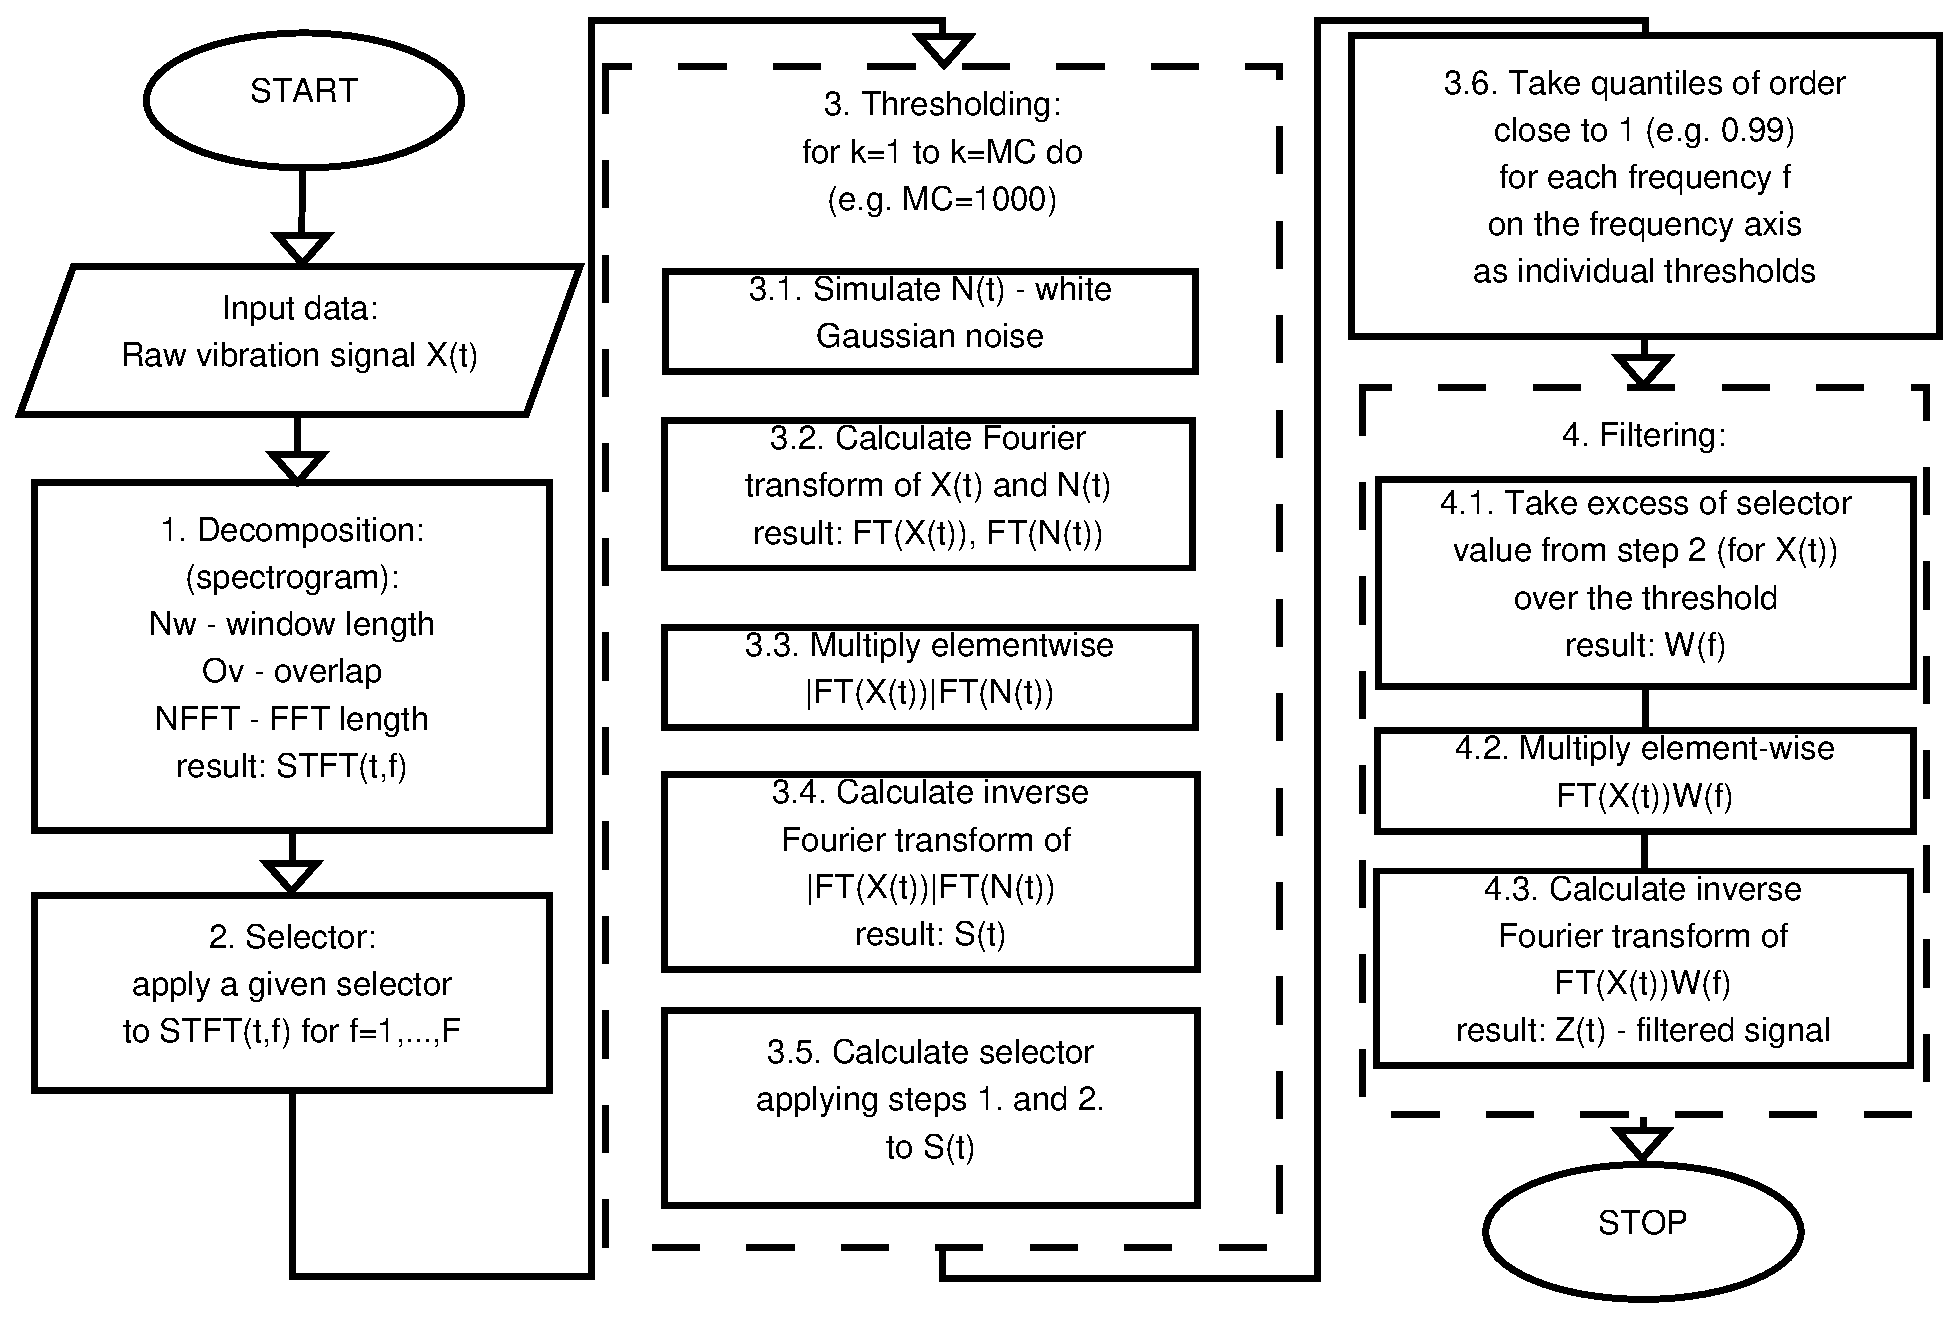
\includegraphics[width=1\textwidth]{Diagram2.eps}
\caption{Block diagram of the filtering procedure.}
\label{diagram}
\end{figure}
\subsection{Decomposition}\label{decomposition}
Decomposition is based on analysis of the discrete short-time Fourier transform (STFT) which for $x_1,x_2,...,x_N$, time point $t= \left\{1,\ldots,T\right\}$ and frequency $f= \left\{1,\ldots,F\right\}$ is defined as follows~\cite{allen}:
\begin{eqnarray}
STFT(t,f)=\sum_{k=0}^{N-1}x_k w(t-k)e^{-2j\pi f k/N},
\label{stft-discr}\end{eqnarray}
where $w(t-k)$ is the shifted window and $x_k$ is the input signal. The window (length and shape) affects the final result in the similar manner as in the spectral kurtosis case. In this paper we present results obtained by using 80\% overlapping.
\subsection{Selectors}\label{selectors}
In this section we recall four selectors~\cite{SelectorsMSSP,bib04}, each of them could be a base for a linear filter. For comparison, one of the selectors is the classical spectral kurtosis. Recall, that the SK is based on the fourth-order statistic. The spectral kurtosis at the frequency bin $f$ is defined as follows~\cite{Antoni2SK}:
\begin{eqnarray}\label{spectral_kurtosis}
SK(f)=T\frac{\sum_{t=1}^{T}|STFT(t,f)|^4}{(\sum_{t=1}^{T}|STFT(t,f)|^2)^2}.
\end{eqnarray}
Besides the ability of a pulse train detection, the $SK$ is also very sensitive to a single non-informative impulse that might occur, for instance, during the signal acquisition. In the classical definition, the sum in~(\ref{spectral_kurtosis}) is reduced by 2 which stands for a cut-off threshold, i.e. only the values of $SK(f)$ larger than 2 are significant. In our approach such subtraction is not necessary - the thresholding procedure quantifies the significance of each selector's value and takes into account only the excess over the threshold.\\
The second selector is the Jarque-Bera statistic~\cite{bib09,Burnecki}. It is based on both kurtosis and skewness. The $JB$ at $f=1,\ldots,F$ is defined as follows:
\begin{eqnarray}
JB(f)=\frac{T}{6}\left(S(f)^2+\frac{\left(K(f)-3\right)^2}{4}\right),
\end{eqnarray}
where $S(f)$ and $K(f)$ are the empirical skewness and kurtosis, respectively, calculated for a given sub-signal, corresponding to the frequency bin $f$. $JB$ exploits not only the fourth, but the third moment as well, in order to examine gaussianity of the random sample. Thus, it might indicate asymmetry of distribution, which occurs in specific types of damage in rotating machines~\cite{Paajarvi}. The higher value of $JB$, the more the distribution of the sample differs from the Gaussian distribution.\\
The next selector is based on a quantile-quantile plot (QQplot). Vertical and horizontal axes of the QQplot are here related to quantiles of empirical sub-signal's distribution and the standard Gaussian distribution, respectively. The selector quantifies the average distance between markers of QQplot and a reference line defined by first and third quartiles of both distributions~\cite{bib04}. The selector $H_{aver}$ at $f=1,\ldots,F$ is defined as~\cite{SelectorsMSSP}:
\begin{eqnarray}
H_{aver}(f)=\frac{1}{T}\sum_{k=1}^{k=T}{ \left| \widetilde{\Phi}^{-1}\left(\frac{2k-1}{2T} \right) - a S(k,f)-b \right| },
\end{eqnarray}
where $\widetilde{\Phi}^{-1}(\cdot)$ is the inverse of cumulative distribution function of the standard Gaussian distribution, i.e. $$\widetilde{\Phi}(x)=\int^{x}_{-\infty} \! \frac{1}{\sqrt{2\pi}}\exp \left( -\frac{x^2}{2} \right) \, \mathrm{d} x,$$ $S(k,f)$ is the $k$-th value of ascending sorted sub-signal $\{|STFT(t,f)|\}_{t=1,\ldots,T}$, $a=\dfrac{\widetilde{\Phi}^{-1}(0.75)-\widetilde{\Phi}^{-1}(0.25)}{q(f,0.75)-q(f,0.25)}$, $b=\widetilde{\Phi}^{-1}(0.75)-aq(f,0.75)$ and $q(f,p)$ is a $p$-th order quantile of a sub-signal $\{|STFT(t,f)|\}_{t=1,\ldots,T}$. In~\cite{bib04} it is shown that this selector distinguishes healthy from faulty bearing's signal as good as SK does, but $H_{aver}$ defines a different order on the set of sub-signals than $SK$ does. Recall that $H_{aver}$ is scale-invariant, since the distance is measured on the axis corresponding to standard normal distribution. Due to the design of $H_{aver}$, one can notice its robustness to single outlying values. One can consider two signals of different lengths, the same statistical distribution and both of them contain a single outlier of similar level. Then $H_{aver}$ is lower for the longer signal, since the appropriate quartiles and $S(k,f)$'s are similar and the denominator, namely $T$, distinguishes these signals.\\
The next selector incorporates the idea of quantifying the distance between the empirical cumulative distribution function (empirical CDF) of the sub-signal and the CDF of the fitted Gaussian distribution. Specifically, it is a Kolmogorov-Smirnov statistic which is defined as follows~\cite{SelectorsMSSP,bib07,bib08}:
\begin{equation}\label{K-S}
KSS(f)=sup_x\left|ECDF(f,x)-\Phi(f,x)\right|,
\end{equation}
where $\Phi(f,\cdot)$ is the cumulative distribution function of the Gaussian distribution with mean and variance estimated from the sub-signal corresponding to the frequency bin $f$. Therefore this function is given by:
\begin{eqnarray}\label{FF}
\Phi(f,x)=\int^{x}_{-\infty} \! \frac{1}{\sqrt{2\pi\widehat{\sigma}(f)^2}}\exp \left( -\frac{\left(x-\widehat{\mu}(f)\right)^2}{2\widehat{\sigma}(f)^2} \right) \, \mathrm{d} x,
\end{eqnarray}
where $\widehat{\mu}(f)$ is the empirical mean of the sub-signal $\{|STFT(t,f)|\}_{t=1,\ldots,T}$, and $\widehat{\sigma}(f)$ is the empirical standard deviation of $\{|STFT(t,f)|\}_{t=1,\ldots,T}$. Moreover, $ECDF(f,x)$ is the empirical cumulative distribution function calculated for the sub-signal corresponding to the frequency bin $f$:
\begin{eqnarray}\label{ECDF}
ECDF(f,x)=\frac{1}{T}\sum_{t=1}^{T}\mathbf{1}\left\{ |STFT(t,f)|\leq x\right\}.
\end{eqnarray}
In the above definition $\mathbf{1}\{a\leq x\}$ denotes the indicator function, i.e. $\mathbf{1}\{a\leq x\}=1$ if $a\leq x$ and 0 otherwise. This selector is also scale-invariant. Moreover, in opposite to the previous selectors, $KSS$ is bounded since values of both cumulative distribution functions (i.e. $ECDF$ and $\Phi$) are between 0 and 1.\\
The values of a particular selector for the entire spectrum constitute a ground for the amplitude response of the filter. The following sections provide a complete description how to obtain the final filter that might be used to obtain the informative part of the vibration signal.
\subsection{Thresholding}\label{thresholding}
Once the amplitude response of the filter is calculated, it has to be enhanced in order to take into account the significant values of the selector only. We propose to design significance thresholds for each frequency bin individually.
\begin{figure}[!ht]
\begin{center}
\includegraphics[width=0.49\textwidth]{sin_const-quantile_lines_g.eps}
\includegraphics[width=0.49\textwidth]{sin_const-quantile_lines_b.eps}
\includegraphics[width=0.49\textwidth]{sin_const-quantile_99_g.eps}
\includegraphics[width=0.49\textwidth]{sin_const-quantile_99_b.eps}
\caption{Selector values of reference signals. Faulty (right panels) and healthy machine (left panels). Red thick lines represent selector values based on $H_{aver}$. Top panels present quantile lines of orders: 0.1, 0.3, 0.5, 0.7 and 0.9 (black thin lines) obtained upon selector values of 1000 reference signals. Bottom panels present significance thresholds for the selector values, i.e. quantile of order 0.99. Note that only at a few frequency bins selector values for healthy machine exceeds the threshold and the threshold is significantly exceeded at 2000-7000~Hz for faulty machine.\label{sim-selekt}}
\end{center}
\end{figure}
This step is essential when energy contained in the informative frequency band is relatively low, i.e. the signal also contains high-energy components that do not carry information about the local damage. In order to illustrate this point, consider a vibration signal that consists of: a) high-energy low-frequency component (component related to normal operation of the machine), b) low-energy component located at the half of the frequency range (component related to local damage) and c) low-energy noise located at the highest frequency bands (non-informative from diagnostic point of view). Values of any selector (that indicates impulsivity) at low frequency bands (not related to damage) are significantly lower than selector values at middle frequency bands (related to local damage). Thus, the signal filtered using such selector might still be affected by the low-frequency component. In other words, high spectral amplitudes of low-frequency signal components multiplied by low selector values might be still larger than low amplitudes (located at informative, middle frequency bands) multiplied by a high values of the selector. Thus, the whole procedure might provide unsatisfactory results, i.e. energy of non-informative components will dominate in the filtered signal.\\
Another reason describing benefits of thresholding is derived from analysis of a signal that consists of the high-energy low-frequency component and the noise only. It might happen that selector values at low frequency bands, containing high-energy  deterministic content, are different from values at frequency bands containing noise (with relatively low energy). Such case might be caused by specific windowing, e.g. when the STFT window length is not large enough to appropriately estimate energy flow at low frequency bands. Fig.~\ref{sim-selekt} illustrates this point. The signals $r_1(t)$ and $r_2(t)$ presented therein are sums of 6 sine waves with frequencies $190n$~Hz, $n=1,\ldots,6$ and a noise dependent on whether the signal from faulty or healthy machine is simulated. The signals $\left\{r_k(t)\right\},\,k=1,2$ are obtained using the following formula:
\begin{eqnarray}
r_k(t)=\sum^{N}_{n=1}{ A a_n \sin(2\pi f_n t)} + \sigma m_k(t),
\end{eqnarray}
where $N=6$, $A=10$, $a_n=0.75^{(n-1)}$, $f_n=190n$, $\sigma=0.1$ and $\left\{m_k(t)\right\},\,k=1,2$ is the noise. The signal from a healthy machine corresponds to the noise $m_1(t)$, which basically is a zero-mean white Gaussian noise with standard deviation equal to 1. $m_2(t)$ is related to a faulty machine and structure of this signal is more complicated. In order to construct $m_2(t)$ we decompose the signal $m_1(t)$ by filtering into 3 components: a) $\left\{m_{1a}(t)\right\}$ - low-pass filtered $\left\{m_1(t)\right\}$ with cut-off frequency 2000~Hz, b) $\left\{m_{1b}(t)\right\}$ - bandpass filtered $\left\{m_1(t)\right\}$ with cut-off frequencies 2000~Hz and 7000~Hz and c) $\left\{m_{1c}(t)\right\}$ - high-pass filtered $\left\{m_1(t)\right\}$ with cut-off frequency 7000~Hz. We use ideal filters, i.e. filters with characteristics equal to 1 along the passed band and 0 elsewhere. Then, we modulate amplitude of $\left\{m_{1b}(t)\right\}$ using an impulsive signal - sum of 128 sine waves with frequencies that are multiples of the fault frequency - $13$~Hz. As a result, the amplitude of the signal between impulses becomes similar to the corresponding amplitude of $\left\{m_1(t)\right\}$. Signal to noise ratio defined as $\mathrm{SNR_{dB}} = 10 \log_{10} \left ( \frac{P_\mathrm{signal}}{P_\mathrm{noise}} \right )$, where $P_\mathrm{signal}$ denotes power of $\sigma m_k(t)$ and $P_\mathrm{noise}$ - power of $\sum^{N}_{n=1}{ A a_n \sin(2\pi f_n t)}$, equals to -42.53~dB in healthy case ($m_1(t)$) and -36.21~dB in faulty case ($m_2(t)$). Frequency sampling is $16384$~Hz and length of the signals is $2.5$~s. The time-frequency map that provides sub-signals is calculated using 133-sample-long Kaiser windows ($\beta=5$) and discrete Fourier transform calculated in 512 points. It can be noticed that values of $H_{aver}$ at low frequency bands are different than values of $H_{aver}$ at middle and high frequency bands. Thus, we claim that each single frequency bin should be thresholded individually.\\
The proposed thresholding procedure is inspired by so called "pre-whitening". Pre-whitening is a method that flattens frequency spectrum of the examined signal~\cite{bib10,bib11,bib12}. Formula for the pre-whitened version of a signal $x(t)$ is~\cite{Borghesani2013}:
\begin{equation}
y(t)=IDFT\left\{\frac{DFT\left(x(t)\right)}{\left|DFT\left(x(t)\right)\right|}\right\},
\end{equation}
where $DFT$ and $IDFT$  indicate the discrete Fourier transform and its inverse. Frequency spectrum of a signal processed using pre-whitening is flat, but the signal might still contain spikes related to local damage. When the damage signature is weak, the pre-whitened signal might be dominated by noise from frequency bands outside the informative frequency band. Thus, there is a need for enhancement of the pre-whitened signal.\\
We use an inverse of pre-whitening in order to simulate a large number of signals without transients (so called reference signals), but keeping the amplitude spectrum similar to the real data's frequency spectrum. Basically, we multiply absolute value of discrete Fourier transform of the examined signal (e.g. $r_k(t)$ or real data) element-wise by discrete Fourier transform of white noise, i.e. $DFT\left\{n(t)\right\}$, where $n(t)$ is a vector of independent identically distributed Gaussian random variables with mean $\mu=0$ and variance $\sigma^2=1$. Length of $n(t)$ is the same as length of the examined signal. Then, we return to time domain using inverse discrete Fourier transform. The formula for a simulated signal without transients is:
\begin{equation}
s(t)=IDFT\left\{{\left|DFT\left(p(t)\right)\right|}{DFT\left(n(t)\right)}\right\},
\end{equation}
where $p(t)$ is the examined signal and the multiplication is performed element by element. Next, we calculate values of the selector for each reference signal $s(t)$.\\
The procedure is repeated with a lot (e.g. 1000) of different $n(t)$'s (so called Monte Carlo method), thus we obtain a significant number of selector values for each frequency bin. Finally, a certain quantile (e.g. $99\%$) is calculated individually for every $f$. If the selector value at $f$ is lower than the quantile, it is said to be insignificant and set to 0. Otherwise, only the excess over the quantile is taken for final design of the filter.\\
Fig.~\ref{coloring-stft} in Sec.~\ref{real_data} presents a spectrogram of a vibration signal from a locally damaged heavy rotating machine (a two-stage gearbox from a mining company) and a spectrogram of an exemplary realization of the simulated signal $s(t)$. One can see that both signals share similar content along frequency axis, but the simulated one has no wide-band excitations related to local damage.
\subsection{Filtering}
In the final step we propose to follow the approach presented in~\cite{CombetSK}, where the optimal Wiener filter based on the $SK$ is described. Recall, that the filter is proportional to the square root of the $SK$. We propose to follow this approach to the selectors proposed in Sec.~\ref{selectors} and replace square root of the $SK$ by square root of selector values that remains after filter's amplitude response enhancement (thresholding). We also normalize these square roots by their maxima in order to make visual comparison of them easier.\\
Firstly, the discrete Fourier transform of the examined signal is calculated and the filter's amplitude response obtained in Sec.~\ref{thresholding} is interpolated at all the frequency bins of the discrete Fourier transform. Next, the discrete Fourier transform is multiplied element-wise by the interpolated frequency characteristic. Finally, the inverse discrete Fourier transform is used in order to return to the time domain. The formula for the filtered signal $z(t)$ is as follows:
\begin{equation}
z(t)=IFT\left\{{FT\left(x(t)\right)}{W(f)}\right\},
\end{equation}
where $W(f)$ is the amplitude response of the filter driven by a given selector (e.g. $SK(f)$, $KSS(f)$, $H_{aver}(f)$, etc.), i.e. square root of thresholded values of the selector, interpolated to make the size of $W(f)$ equal to the size of discrete Fourier transform of $x(t)$.
\section{Experiment description}\label{experiment}
In this section we describe setup of an experiment that allows us to verify the methodology proposed in the paper.
\begin{figure}[!ht]
\begin{center}
\includegraphics[width=1\textwidth]{fig1.eps}
\caption{a) scheme of the investigated machine, b) location of the accelerometer.}\label{gearbox}
\end{center}
\end{figure}
The investigated machine is a two-stage gearbox which is a part of a belt conveyor driving station used to transport raw materials in a mining company. Scheme of the driving unit is presented in Fig.~\ref{gearbox} (left panel). The data analyzed in Sec.~\ref{real_data} has been acquired using an accelerometer located as it is presented in Fig~\ref{gearbox} (right panel). Measurements have been performed using Br{\"u}el \& Kj{\ae}r Pulse system. Parameters of data acquisition are presented in Sec.~\ref{real_data}. Amplitudes of mesh components are relatively high, thus impulsive signal related to a local damage might be difficult to observe in the raw signal. The damage that occurred in the machine is related to a tooth's local damage in the gear-wheel mounted on the second (middle) shaft. The fault frequency related to it is approximately 4.1~Hz.
\section{Application to industrial data}\label{real_data}
The signal analyzed in this section has been acquired using an accelerometer and represents $2.5$~s of the system's operation.
\begin{figure}[!ht]
\begin{center}
\includegraphics[width=0.7\textwidth]{y2-raw_signal_timeseries.eps}
\includegraphics[width=0.7\textwidth]{y2-raw_envelope_spectrum.eps}
\caption{Time series (top panel) and envelope spectrum (bottom panel) of the real raw vibration signal from the two-stage gearbox. Red dashed lines denote 14 first multiplies of fault frequency (4.1~Hz).\label{raw-timeseries}}
\includegraphics[width=0.76\textwidth]{y2-raw_signal_spectrogram.eps}
\includegraphics[width=0.76\textwidth]{y2--raw_signal_spectrogram_colored.eps}
\caption{Spectrograms of the raw real (top panel) and one of the reference signals obtained by using the method based on inverse pre-whitening (bottom panel). Note similar frequency content of both signals (e.g. area labeled D). The difference can be noticed in terms of presence of wide-band excitations related to local damage (e.g. labeled SOI$_1$, SOI$_2$).\label{coloring-stft}}
\end{center}
\end{figure}
Sampling frequency is $8192$~Hz.\\
Time series and its envelope spectrum are presented in Fig.~\ref{raw-timeseries}. Impulses related to the local damage are barely visible in time domain due to high-energy low frequency components that do not carry impacts related to damage. The envelope spectrum does not indicate any of multiplies of the fault frequency ($4.1$~Hz). Spectrogram of the signal is presented in Fig.~\ref{coloring-stft} (top panel). Bottom panel of Fig.~\ref{coloring-stft} presents an exemplary reference signal. Recall, that this signal is basically a white Gaussian noise with amplitude spectrum multiplied by the spectrum of real data. Parameters of the STFT are: Kaiser window of length 329~samples, $80\%$~overlapping and the discrete Fourier transform is calculated in 1024~points. Time-frequency map of the real data exhibits a few wide-band excitations, a single artifact which is invisible in time domain and high-energy low-frequency components. The artifact can be easily noticed in the spectrogram at highest frequency bands, i.e. over $3500$~Hz. One can see that the most informative frequency band is located around $1000$~Hz, but some wide-band excitations can be also seen close to $250$~Hz and $2800$~Hz (Fig.~\ref{coloring-stft}). This behavior is a result of the resonance effect - informative frequency band consists of two or more separated informative frequency sub-bands.\\
\begin{figure}[!ht]
\begin{center}
\includegraphics[width=0.49\textwidth]{y2-selector-0.eps}
\includegraphics[width=0.49\textwidth]{y2-selector-7.eps}
\includegraphics[width=0.49\textwidth]{y2-selector-3.eps}
\includegraphics[width=0.49\textwidth]{y2-selector-1.eps}
\caption{Filter characteristics before thresholding (red thick lines) and significance thresholds (black thin lines), a) $SK$, b) $JB$, c) $KSS$, d) $H_{aver}$.\label{f:selectors}}
\end{center}
\end{figure}
Selector values and significance thresholds corresponding to each of four selectors are compared in Fig.~\ref{f:selectors}. One can notice that the artifact has the most significant influence on $JB$ and $SK$, but the rest of the selectors are also slightly influenced. Thus, signal processing methods based on finding frequency band with the highest kurtosis or, in general, highest value of a given selector will definitely fail, since it will result in a signal with the artifact and low-energy noise. This is the reason why all of the frequency bins with significantly high selector values have to be taken into account in the signal filtering procedure. Otherwise, a bandpass filter with center frequency corresponding to the maximum of the selector's values might omit remaining features, assessed as significant. Characteristics of the filters based on $KSS$ and $H_{aver}$ are the least sensitive to the single disturbance. Moreover, values of $H_{aver}$ at highest frequency bands are close to values at middle-low bands (about 1000~Hz) (Fig.~\ref{f:selectors}). The plots also illustrate the relevance of individual significance thresholds for each frequency bin.  At several frequency bins related to frequencies lower than 1000~Hz, the thresholds significantly differ. Thus, it cannot be said that a flat threshold (i.e. the same for each $f$) is appropriate. Higher values of selectors at the lowest frequency bins might have the same cause as in the simulated signals presented in~\ref{sim-selekt}. The problem of alternative methods for assessment of significance (thresholding) is investigated in Sec.~\ref{discussion}.\\
Time series of filtered signals are presented in Fig.~\ref{f:timeseries_filtered}. It can be noticed that the artifact occurred only in case of $SK$ and $JB$. Recall, that both of them are based on statistical moments. Other selectors, based on sample quantiles ($H_{aver}$) and empirical cumulative distribution function ($KSS$), suppressed the artifact to the level of noise. In all of 4 selectors, spikes related to local damage are now cleary visible in time domain.\\
\begin{figure}[!ht]
\begin{center}
\includegraphics[width=0.45\textwidth]{y2-timeseries-0.eps}
\includegraphics[width=0.45\textwidth]{y2-timeseries-7.eps}
\includegraphics[width=0.45\textwidth]{y2-timeseries-3.eps}
\includegraphics[width=0.45\textwidth]{y2-timeseries-1.eps}
\caption{Time series of filtered vibration signals, a) $SK$, b) $JB$, c) $KSS$, d) $H_{aver}$. Time point at which the artifact occurs is marked by ellipse.\label{f:timeseries_filtered}}
\includegraphics[width=0.45\textwidth]{y2-envelope_spectrum-0.eps}
\includegraphics[width=0.45\textwidth]{y2-envelope_spectrum-7.eps}
\includegraphics[width=0.45\textwidth]{y2-envelope_spectrum-3.eps}
\includegraphics[width=0.45\textwidth]{y2-envelope_spectrum-1.eps}
\caption{Envelope spectra of filtered vibration signals, a) $SK$, b) $JB$, c) $KSS$, d) $H_{aver}$. Red dashed lines correspond to first 14 multiplies of fault frequency (4.1~Hz).\label{f:spectra_filtered}}
\end{center}
\end{figure}
Envelope spectra of filtered signals are presented in Fig.~\ref{f:spectra_filtered}. It is shown that the relatively low-energy artifact that occurred during the experiment has affected characteristics of filters. However, the amplitude of the artifact is not high enough to affect envelope spectra of filtered signals. In all cases the fault frequency is properly recognized as 4.1~Hz. Lots of multiples of the fault frequency can be noticed.
\section{Influence of larger artifact on filtered signal}\label{artifact_influence}
Here we present how our procedure deals with a simulated signal with a larger artifact.
\begin{figure}[!ht]
\begin{center}
\includegraphics[width=1\textwidth]{y4colored-raw_signal_timeseries.eps}
\caption{Time series of: a) the raw real vibration signal, b) simulated impulsive signal, c) artifact, d) sum of above signals.\label{y4-timeseries}}
\end{center}
\end{figure}
\begin{figure}[!ht]
\begin{center}
\includegraphics[width=1\textwidth]{y4colored-raw_signal_spectrogram.eps}
\caption{Spectrogram of the raw signal. Informative frequency band (3800-4200~Hz) and the artifact are marked by rectangle labeled "SOI" and marked by ellipse, respectively.\label{y4-coloring-stft}}
\end{center}
\end{figure}
The signal is obtained by compiling frequency structure from a signal that represents vibrations of a healthy heavy rotating machine, simulated signal of interest and the artifact. The machine is of the same kind as in the previous section (two-stage gearbox operating in the driving station for belt conveyor), but the sensor (accelerometer) is located on a different place on the housing. Thus, frequency structures of both signals are different. Moreover, sampling frequency of the signal is now 16384~Hz and duration is 2.5~s. The simulated signal of interest is an amplitude modulated Gaussian noise and it imitates a pulse train related to a local damage of the first shaft. Moreover, the pulse train is band-passed using an ideal filter to obtain relatively narrow informative frequency band, i.e. 3800-4200~Hz, which is typical for the local damage in early stage. Fault frequency is equal to 16.5~Hz. Also a single impulse is added in order to simulate an artifact. The impulse is short-lasting, but its amplitude is relatively high. We simulated the impulse as a Gaussian-modulated sinusoidal pulse. Its bandwidth completely covers the bandwidth of the SOI. Moreover, it covers almost the entire frequency range. The finally analyzed signal is a sum of these 3 signals.\\
Time series of all components of the signal are presented in Fig.~\ref{y4-timeseries}. The spectrogram of the analyzed signal is presented in Fig.~\ref{y4-coloring-stft}. The spectrogram is obtained by using Kaiser windows of length 223 samples, $80\%$ of overlapping and the discrete Fourier transform is calculated in 512 points.\\
The signal is designed to clearly illustrate how relevant it is to minimize the influence of a single artifact on frequency characteristic of a filter. In the previous case the artifact was too small to illustrate this statement, thus the analysis of the simulated signal is performed.\\
\begin{figure}[!ht]
\begin{center}
\includegraphics[width=0.49\textwidth]{y4colored-selector-0.eps}
\includegraphics[width=0.49\textwidth]{y4colored-selector-7.eps}
\includegraphics[width=0.49\textwidth]{y4colored-selector-3.eps}
\includegraphics[width=0.49\textwidth]{y4colored-selector-1.eps}
\caption{Filter characteristics before cut-off (red thick lines) and thresholds (black thin lines), a) $SK$, b) $JB$, c) $KSS$, d) $H_{aver}$.\label{f:selectors-y4}}
\end{center}
\end{figure}
Fig.~\ref{f:selectors-y4} presents characteristics of filters based on $SK$, $JB$, $KSS$ and $H_{aver}$. It can be seen that the artifact influenced all of the selectors. Similar to the previous case (real data, Sec.~\ref{real_data}), the artifact influenced frequency characteristic driven by $JB$ the most, the next is $SK$ (both of them are based on statistical moments). $KSS$ and $H_{aver}$ are barely influenced. It is worth pointing out that the idea of individual significance thresholds for each frequency bin has been proved as important. There is a peak in the lowest frequency bands, clearly visible in Fig.~\ref{f:selectors-y4}, panels c) and d), but also in panel a). Any amount of this low-frequency high-energy part of the signal not suppressed by the filter might result in worsening of quality of the filtered signal.\\
\begin{figure}[!ht]
\begin{center}
\includegraphics[width=0.49\textwidth]{y4colored-timeseries-0.eps}
\includegraphics[width=0.49\textwidth]{y4colored-timeseries-7.eps}
\includegraphics[width=0.49\textwidth]{y4colored-timeseries-3.eps}
\includegraphics[width=0.49\textwidth]{y4colored-timeseries-1.eps}
\caption{Time series of filtered simulated signals, a) $SK$, b) $JB$, c) $KSS$, d) $H_{aver}$. Time point at which the artifact occurs is marked by ellipse.\label{f:timeseries_filtered-y4}}
\includegraphics[width=0.49\textwidth]{y4colored-envelope_spectrum-0.eps}
\includegraphics[width=0.49\textwidth]{y4colored-envelope_spectrum-7.eps}
\includegraphics[width=0.49\textwidth]{y4colored-envelope_spectrum-3.eps}
\includegraphics[width=0.49\textwidth]{y4colored-envelope_spectrum-1.eps}
\caption{Envelope spectra of filtered simulated signals, a) $SK$, b) $JB$, c) $KSS$, d) $H_{aver}$. Red dashed lines denote 7 first harmonics of the fault frequency (16.5~Hz).\label{f:spectra_filtered-y4}}
\end{center}
\end{figure}
Time series of the filtered signals are presented in Fig.~\ref{f:timeseries_filtered-y4}. It can be easily noticed that the artifact is present in every plot, but its amplitude depends on a particular selector. The frequency bands of SOI are completely covered by the frequency band of the artifact. Thus, it is impossible to completely remove the artifact from the filtered signal, using a linear filter based on suppressing selected frequency bins. One can only design a filter that minimizes amplitude of the accidental impulse by suppressing energy of all other frequency bins that do not contain the SOI. In Fig.~\ref{f:timeseries_filtered-y4} one can observe that in panel a) impulses related to the signal of interest are barely visible and in panel b) they are completely invisible. On the other hand, impulses might be clearly seen in panels c) and d) of Fig.~\ref{f:timeseries_filtered-y4} and amplitude of the artifact is comparable to the amplitude of impulses that constitutes the SOI. $KSS$ and $H_{aver}$ indicated almost only the frequency band of the SOI, thus the noise at frequency bands under 3800~Hz and above 4200~Hz is minimized. Therefore, the resultant signals are close to the SOI presented in panel b) of Fig.~\ref{y4-timeseries}. Bandwidth of the artifact is highly reduced, thus its amplitude is diminished as well.\\
As it was expected after the analysis presented in the previous section, single spike influenced envelope spectra the most in two of four cases ($SK$ and $JB$ - Fig.~\ref{f:spectra_filtered-y4}, panels a) and b), respectively). The envelope of the $SK$-filtered signal contains one peak corresponding to the fault frequency (16.5~Hz) with large amount of noise (Fig.~\ref{f:spectra_filtered-y4}). Panel b) of Fig.~\ref{f:spectra_filtered-y4}, which represents the result of filtration using $JB$, contains only a noise - none of fault frequency harmonics is presented. On the other hand, filters based on $KSS$ and $H_{aver}$ (Fig.~\ref{f:spectra_filtered-y4}, panels $c)$ and $d)$, respectively) recognized the true fault frequency, showing three clear harmonics related to first 3 multiples of the fault frequency. Also, the level of the noise is much lower in these two cases.\\
To sum up, the best results are obtained by filtering using selectors based on quantiles and empirical cumulative distribution function, i.e. $H_{aver}$ and $KSS$, respectively. Signals filtered using selectors based on statistical moments are very sensitive to accidental impulses, thus they fail in case of the artifact.
\section{Discussion}\label{discussion}
In this section we discuss motivation and properties of the proposed methodology and compare it with existing methods. The novelty of the paper is contained mainly in the extension of SK-based filtering (including the thresholding procedure), thus we discuss other methods of one dimensional clustering that might be found in the literature. One dimensional methods of clustering are significantly different from multidimensional ones. The 1D real-valued data is only a special case of multidimensional data, but the difference is in natural ordering of real numbers. All of the discussed methods benefit from this property. The fundamental problem is to distinguish between significant and insignificant values of a particular selector. Thus, there is a need for clustering values of the selector into two groups only.\\
The classical approach for filtering based on the spectral kurtosis (calculated from the STFT) is to subtract 2 from calculated fourth-order statistic and then take only excess over a given significance level $\alpha$, which is proportional to the given quantile of the normal distribution~\cite{CombetSK,Antoni2SK}. While applying other impulsivity criteria (selectors) to the signal, one can derive analogous thresholds for each single selector. On the other hand, one can simply exploit one of the existing 1D thresholding procedures. We recall and analyze only a few of them, because comparing thresholding methods is not the goal of this paper.\\
In 1979 N. Otsu proposed a method for finding the threshold that minimizes the variance within the group, namely a weighted sum of each group's variances, where weights are just the number of elements in a particular group divided by the number of all thresholded values~\cite{Otsu}. In order to calculate this variance-minimizing threshold it is proposed to calculate firstly the variance within the group, taking as the threshold each element of the entire set in the sequence. Then, the final threshold is the argument which minimizes the variance within the group. In our case, where the entire set of selector values is denoted by $\left\{W(f),\,f\in \left\{ 1,\ldots,F\right\}\right\}$ it is only needed to calculate, for each $f_i\in \left\{ 1,\ldots,F\right\}$, the weighted average of variances of each of two groups - one constituted from elements of $\left\{W(f)\leq W\left(f_i\right),\,f\in \left\{ 1,\ldots,F\right\}\right\}$  and $\left\{W(f) > W\left(f_i\right),\,f\in \left\{ 1,\ldots,F\right\}\right\}$. Then, $f_i$ that maximized the weighted sum of variances is the final threshold. Such method is known for setting the threshold close to the component with larger class probability or larger class variance~\cite{MinVarThresholding}, thus it might fail if only a small frequency band is non-informative (with low values of $W(f)$) and values of $W(f)$ at other frequency bands are much higher and scattered. Then, the threshold might be too high, what results in ignoring some of the informative frequency bins. Recently, a new method for such heavy-tailed 1D data classification called "head/tail breaks" has been proposed by B. Jiang~\cite{HeadTailBreaks}. In order to avoid the effect of threshold shifting through the right tail of the data, it is proposed to iteratively constitute breakpoints (thresholds). Each breakpoint divides a set into two subsets - one above and one below the breakpoint. These breakpoints are just arithmetic means of the considered set, thus in the first step the arithmetic mean $\mu_1$ of all values in $\left\{W(f),\,f\in \left\{ 1,\ldots,F\right\}\right\}$ is calculated. Then, the mean $\mu_2$ of values above $\mu_1$ is calculated, and so on. In our case, where $\left\{W(f),\,f\in \left\{ 1,\ldots,F\right\}\right\}$ has to be divided into two groups only, this method might provide unsatisfactory results when, for instance, there are just a few values of the selector at IFB much higher than others therein, and low values at non-informative frequency band are present, as usual. Arithmetic mean is known to be sensitive to outliers, thus, once again, some of informative components might be omitted. To sum up, both methods are interesting since they do not assume specific distribution of the data. However, they might omit some informative components, for which corresponding values of the selector are not the largest, but still are significant. This remark led us to invent the thresholding method described in Sec.~\ref{thresholding}. This one might be applied not only to the kurtosis calculated from the spectrogram, but also to other selectors, for which taking a given quantile of Gaussian distribution is not a method proved as efficient. The only thing we assume is that the reference signal which imitates the same signal as the investigated one, but without local damage, might be simulated using the inverse pre-whitening. Using a number of such simulated signals it can be examined, whether our investigated machine significantly differs from a healthy one or not. Additional advantage of this method is its insensitivity to windowing, i.e. when a particular STFT windowing method provides unlikely high values of a selector for some frequency bands, the method adapts and makes the threshold higher at these bands. One can also make the procedure closer to the reality, i.e. when an appropriate (large) number of signals representing the same measurement related to a healthy machine, might be acquired. Since this extension might be performed well in a laboratory, its application to an industrial case might be difficult.
\section{Conclusions}
In this paper a new technique for noisy vibration signals enhancement has been presented in application to local damage detection in rotating machinery. It is based on extension of the SK-based filtering procedure, where the SK is substituted by several selectors. Moreover, the novel significance assessment procedure (thresholding) has been introduced as a method for filter's amplitude response enhancement. The procedure is based on inverse pre-whitening and exploits Monte Carlo method. It was shown that the technique might provide more effective results, particularly in industrial conditions where a vibration signal might contain impulses not related to any kind of damage. If the frequency bands of an isolated impact and the SOI are disjoint, then our procedure minimized amplitude of the artifact to the amplitude of noise. In another case, i.e. when the IFB is totally covered by the frequency band of the isolated impact, amplitude of the artifact has been suppressed to the amplitude of the SOI.\\
In the literature one can find several other methods that might deal with thresholding, although the one based on inverse pre-whitening seems to posses all of the suitable properties. The thresholding proposed in this paper might be extended by using the real vibration signals only, but such extension to industrial conditions is disputable, since it a large number of reference signals is difficult to obtain.
\section{Conflict of Interests}
The authors declare that there is no conflict of interests
regarding the publication of this paper.

\begin{thebibliography}{00}
\bibitem{Surveillance7} J. Obuchowski, A. Wylomanska, R. Zimroz, Novel enhancement techniques for noisy vibration signals applied to local damage detection in rotating machines, paper presented at "The International Conference Surveillance 7", Chartres, France, October 29-30, 2013.
\bibitem{Kia2015} S.H. Kia, H. Henao, G.-A. Capolino, "Gear Tooth Surface Damage Fault Detection Using Induction Machine Stator Current Space Vector Analysis" IEEE Trans. Ind. Electron. 62 (3) (2015) 1866-1878.
\bibitem{EnvelopeNoiseGPU} Myeongsu Kang; Jaeyoung Kim; Jong-Myon Kim, "High-Performance and Energy-Efficient Fault Diagnosis Using Effective Envelope Analysis and Denoising on a General-Purpose Graphics Processing Unit", IEEE Trans. Power Electron. 30 (5) (2015) 2763-2776.
\bibitem{Schur} R.A. Makowski, R. Zimroz, "Adaptive bearings vibration modelling for diagnosis", Lecture Notes in Computer Science (including subseries Lecture Notes in Artificial Intelligence and Lecture Notes in Bioinformatics) 6943 LNAI (2011) 248-259.
\bibitem{Wavelets}  P.W. Tse, W.X. Yang, H.Y. Tam, "Machine fault diagnosis through an effective exact wavelet analysis", J. Sound Vib. 277 (4-5) (2004) 1005-1024.
\bibitem{LocalMaxima} J. Obuchowski, A. Wylomanska, R. Zimroz, "The local maxima method for enhancement of time-frequency map and its application to local damage detection in rotating machines", Mech. Syst. Signal Process. 46 (2) (2014) 389-405.
\bibitem{BurdzikSHM} R. Burdzik, L. Konieczny, P. Folega, "Structural health monitoring of rotating machines in manufacturing processes by vibration methods", Advanced Materials Research 1036 (2014) 642-647.
\bibitem{ZakMS} G. Zak, J. Obuchowski, A. Wylomanska, R. Zimroz, "Novel 2D representation of vibration for local damage detection", Mining Science 21 (2014) 21, 105-113.
\bibitem{Leite} V.C.M.N. Leite, J.G. Borges Da Silva, G.F.C. Veloso, L.E. Borges Da Silva, G. Lambert-Torres, E.L. Bonaldi, L.E. De Lacerda De Oliveira, "Detection of localized bearing faults in induction machines by spectral kurtosis and envelope analysis of stator current", IEEE Trans. Ind. Electron. 62 (3) (2015) art. no. 6871315, 1855-1865. 
\bibitem{Prieto} M.D. Prieto, G. Cirrincione, A.G. Espinosa, J.A. Ortega, H. Henao, "Bearing fault detection by a novel condition-monitoring scheme based on statistical-time features and neural networks", IEEE Trans. Ind. Electron. 60 (8) (2013) art. no. 6307844, 3398-3407. 
\bibitem{CombetSK} F. Combet, L. Gelman, "Optimal filtering of gear signals for early damage detection based on the spectral kurtosis", Mech. Syst. Signal Process. 23 (3) (2009) 652-668.
\bibitem{Antoni2SK} J. Antoni, R.B. Randall, "The spectral kurtosis: application to the vibratory surveillance and diagnostics of rotating machines", Mech. Syst. Signal Process. 20 (2) (2006) 308-331.
\bibitem{Immovilli}  F. Immovilli, M. Cocconcelli, A. Bellini, R. Rubini, "Detection of generalized-roughness bearing fault by spectral-kurtosis energy of vibration or current signals", IEEE Trans. Ind. Electron. 56 (11) (2009) 4710-4717.
\bibitem{Liu} Z. Liu,, Q. Zhang, "An approach to recognize the transient disturbances with spectral kurtosis", IEEE Trans. Instrum. Meas. 63 (1) (2014) art. no. 6583959, 46-55.
\bibitem{Fournier} E. Fournier, A. Picot, J. Regnierl, M.T. Yamdeu, J.-M. Andrejak, P. Maussion, "On the use of Spectral Kurtosis for diagnosis of electrical machines," in Diagnostics for Electric Machines, Power Electronics and Drives (SDEMPED), 2013 9th IEEE International Symposium on, (2013) 77-84.
\bibitem{CorrKurtosisJVE} X. Zhang, J. Kang, J. Zhao, J. Zhao, H. Teng, "Rolling element bearings fault diagnosis based on correlated kurtosis kurtogram", Journal of Vibroengineering, 17 (6) (2015) 3023-3034.
\bibitem{AntoniKurtogram} J. Antoni, "Fast computation of the kurtogram for the detection of transient faults", Mech. Syst. Signal Process. 21 (1) (2007) 108-124.
\bibitem{Protrugram} T. Barszcz, A. Jablonski, "An enhanced Kurtogram method for fault diagnosis of rolling element bearings", Mech. Syst. Signal Process. 25 (1) (2011) 431-451.
\bibitem{Wavelet_kurtogram}  P.H. Nguyen, J.-M. Kim, "Multifault diagnosis of rolling element bearings using a wavelet kurtogram and vector median-based feature analysis", Shock and Vibration 2015 (2015), art. no. 320508.
\bibitem{Infogram} J. Antoni, "The infogram: Entropic evidence of the signature of repetitive transients", Mech. Syst. Signal Process. (2015), Article in Press.
\bibitem{SelectorsMSSP} J. Obuchowski, A. Wylomanska, R. Zimroz, "Selection of informative frequency band in local damage detection in rotating machinery", Mech. Syst. Signal Process. 48 (1-2) 2014, 138-152.
\bibitem{bib04} J. Obuchowski, A. Wylomanska, R. Zimroz, "Stochastic modeling of time series with application to local damage detection in rotating machinery", Key Eng. Mater. 569-570 (2013) 441-448.
\bibitem{allen} J.B. Allen, "Short term spectral analysis, synthesis, and modification by discrete Fourier transform", IEEE Trans. Acoust. Speech Signal. Process. 25 (3) (1977) 235-238.
\bibitem{bib09} C.M. Jarque, A.K. Bera, "Efficient tests for normality, homoscedasticity and serial independence of regression residuals", Econ. Lett. 6 (3) (1980) 255-259.
\bibitem{Burnecki} K. Burnecki, A. Wylomanska, A. Beletskii, V. Gonchar, A. Chechkin, "Recognition of stable distribution with Levy index alpha close to 2", Phys. Rev. E 85 (5) (2012) 056711. 
\bibitem{Paajarvi} A.K. Ovacikli, P. Paajarvi, J.P. LeBlanc, "Skewness as an objective function for vibration analysis of rolling element bearings", In Image and Signal Processing and Analysis (ISPA) 2013, 8th International Symposium on, (2013) 462-466.
%\bibitem{bib06} R.F. Dwyer, Use of the kurtosis statistic in the frequency domain as an aid in detecting random signals, IEEE J. Ocean. Eng. 9 (2) (1984) 85-92.
\bibitem{bib07} G.W. Corder, D.I. Foreman, "Nonparametric Statistics for Non-Statisticians: A Step-by-Step Approach", Wiley 2009.
\bibitem{bib08} A. Justel, D. Pen, R. Zamar, "A multivariate Kolmogorov-Smirnov test of goodness of fit", Statist. Probab. Lett. 35 (3) (1997) 251-259.
\bibitem{bib10} N. Sawalhi, R.B. Randall, "Spectral kurtosis enhancement using autoregressive models", 4th Australasian Congress on Applied Mechanics, 2005, 231-236. 
\bibitem{bib11} N. Sawalhi, R.B. Randall, "Signal pre-whitening for fault detection enhancement and surveillance in rolling element bearings", Paper presented at the Eighth International Conference on Condition Monitoring and Machinery Failure Prevention Technologies, St David's Hotel, Cardiff, UK, 2011, 20-22 June.
\bibitem{bib12} N. Sawalhi, R.B. Randall, "Vibration response of spalled rolling element bearings: Observations, simulations and signal processing techniques to track the spall size", Mech. Syst. Signal Process. 25 (3) (2011) 846-870.
\bibitem{Borghesani2013} P. Borghesani, P. Pennacchi, R.B. Randall, N. Sawalhi, R. Ricci, "Application of cepstrum pre-whitening for the diagnosis of bearing faults under variable speed conditions", Mech. Syst. Signal Process. 36 (2) (2013) 370-384.
\bibitem{Otsu} N. Otsu, "A threshold selection method from gray-level histograms", IEEE Trans. Sys., Man., Cyber. 9 (1) (1979) 62-66.
\bibitem{MinVarThresholding} Z. Hou, Q. Hu, W.L. Nowinski, "On minimum variance thresholding", Pattern Recogn. Lett. 27 (14) (2006) 1732-1743.
\bibitem{HeadTailBreaks} B. Jiang, "Head/Tail Breaks: A New Classification Scheme for Data with a Heavy-Tailed Distribution", Prof. Geogr. 65 (3) (2013) 482-494.

\end{thebibliography}


\end{document}
